\section{Introduction}\label{sec:intro}

\paragraph{Motivation.} Thin composite panels stiffen as they vibrate. Mid-plane
stretching makes the restoring force of a bending mode cubic in its amplitude, so the
resonance frequency drifts upward with amplitude along the \emph{backbone curve}
$\Om(a)$ \cite{touze,shaw}. Under harmonic forcing, the hardening resonance leans over,
folds, and \emph{jumps} between coexisting branches with hysteresis. For a resonant
sensor the drift is a calibration error. For a harvester or an actuator the jump is a
loss of function. In practice, the designer of such a panel is not free to move its
linear frequency (set by the application) or its mass (set by the vehicle). The design
question is therefore whether the \emph{nonlinear} stiffness can be changed
\emph{independently} of both.

\subsection{Related work and positioning}\label{sec:related}
\paragraph{Reduction and design of nonlinear normal modes.} The backbone is the
frequency--amplitude relation of a nonlinear normal mode \cite{shaw,kerschen2009,nayfeh1979}.
Spectral submanifold (SSM) theory makes it the reduced dynamics on the unique smoothest
invariant manifold tangent to a modal subspace \cite{haller2016}. Its parametrization can
be computed directly from finite-element models to arbitrary order
\cite{ponsioen2018,jain2022,vizzaccaro2022,opreni2023}; see \cite{touze} for a review of
geometrically nonlinear reduction. This makes nonlinear response a \emph{designable}
quantity. Dou et al.\ shaped normal-form coefficients of beams and frames by adjoint
shape optimization \cite{dou2015,doujensen2016}. Li derived explicit SSM sensitivities
\cite{li2024}. Pozzi et al.\ tailored conservative backbones through the reduced dynamics of
Lyapunov subcenter manifolds \cite{pozzi2024lsm}, obtained adjoint sensitivities of SSM
backbone curves at arbitrary order \cite{pozzi2025}, and optimized the topology of the
hardening/softening coefficient \cite{pozzi2025smo}. Liang et al.\ extended adjoint SSM
sensitivities to forced-response curves and density-based topology optimization
\cite{liang2025}. Force-based reduced-order models have also been used to optimize
nonlinear finite-element models \cite{xiao2026}. These works supply the tools we use
(SSM reduction, adjoint sensitivities, gradient-based design), and we claim no novelty for
them. Their design variables are the \emph{shape}, \emph{size} or \emph{material density} of
isotropic structures. None uses a fiber-orientation field, and none imposes the tow-curvature
limit of automated fiber placement.

\paragraph{Variable-stiffness composites.} Steering tows along curvilinear paths was
introduced for buckling and stress concentration \cite{hyer1991}. It is now a mature design
space for \emph{linear} objectives: in-plane stiffness and buckling
\cite{gurdal,lopes2008,ijsselmuiden}, and fundamental frequency through lamination
parameters \cite{abdalla2007,tsai1968}, including manufacturable segmentations of the
optimal stiffness field \cite{sheikhi2024} and layer-wise frequency optimization that
models the gaps and overlaps of tow placement \cite{pagani2025,fayazbakhsh2013}. Steering has
also been optimized for a geometrically nonlinear \emph{static} objective, postbuckling stiffness
\cite{wu2013,raju2018}, where the gain is attributed to the in-plane redistribution of load
toward the supported edges \cite{gurdal,wu2013}; the relaxed-stretch mechanism identified
here is closely analogous. Orientation is also optimized pointwise in topology-optimization
frameworks \cite{stegmann2005,nomura2015}, and continuous-fiber printing \cite{matsuzaki2016}
with toolpath-integrated, curvature-constrained design \cite{wong2026} lays such fields
directly. The \emph{nonlinear} vibration of variable-stiffness plates has been
\emph{analyzed} for \emph{prescribed} fiber paths: linear modes \cite{akhavan2011}, forced
periodic vibrations \cite{akhavan2015,akhavan2017} and free nonlinear vibrations
\cite{ribeiro2012,ribeiroakhavan2012} (Akhavan and Ribeiro), nonlinear free vibration
\cite{houmat2013}, semi-analytical parametric studies of free and forced response
\cite{yan2021}, and, most recently, backbone curves in a thermal environment with a
higher-order shell element \cite{zhao2026}. The nearest neighbor is the work of Farsadi et
al.\ \cite{farsadi2021,farsadi2025}. They optimize curvilinear fiber paths for the
\emph{linear} fundamental frequency and then examine the amplitude-dependent frequency of the
optimum.

\paragraph{What is new here.} Relative to \cite{farsadi2021,farsadi2025}, the objective is
the nonlinear hardening coefficient itself, minimized \emph{under an equality constraint on
the linear frequency} at fixed mass, rather than the frequency with the nonlinear response
assessed afterwards. Relative to the SSM-optimization literature, the design variable is a
fiber-orientation field under the pointwise tow-curvature limit, with the material and its
mass fixed. The central contribution is not the optimizer but a \emph{mechanism}: two
strain fields of one mode weight the same anisotropic stiffness differently. A local Fourier
theory then predicts when steering must help, where the fibers go and what limits the gain.
Each prediction is tested against the competing laminate freedoms, a uniform angle and the
stacking sequence, by comparing the attainable (frequency, hardening) sets.

\paragraph{Why it matters.} Designers of resonant devices already exploit or cancel
geometric nonlinearity by tuning design parameters, for example by balancing mechanical
hardening against electrostatic softening to extend the linear range of nanomechanical
sensors \cite{kacem2009}. A composite panel offers an additional freedom that leaves
geometry, mass and material unchanged.

\begin{center}
\fbox{\begin{minipage}{0.94\linewidth}\small
\textbf{The design quantity $J$, operationally.} For the panel's fundamental mode with
mid-plate deflection amplitude $a$ (in meters), the backbone to cubic order is
\[
\frac{\Om(a)}{\omega_1}=1+\tfrac38\,J\,a^2,\qquad J=\frac{\gamma}{\omega_1^2\,w_c^2}\ \ [\mathrm m^{-2}],
\]
where $\gamma$ is the cubic coefficient of the single-mode reduced dynamics
$\ddot q+\omega_1^2q+\gamma q^3=0$ and $w_c$ the mode's mid-plate value (Sec.~\ref{sec:model}).
$J$ does not depend on the mode normalization, and $\tfrac38Ja^2$ is the relative frequency shift
that a ring-down or a stepped-sine test measures at amplitude $a$. A ratio
$J/J_{\UD}=0.37$ means that, at the same amplitude, the frequency drifts $37\%$ as much as
in the unidirectional (UD) panel. Equivalently, the same drift is reached at
$(0.37)^{-1/2}=1.65$ times the amplitude. For the UD plate studied here
($200\times150\times2$\,mm, simply supported), $f_1=\nUDf$\,Hz and the shift is
$\nUDdet\%$ at $a=0.4h=\SI{0.8}{mm}$.
\end{minipage}}
\end{center}

\paragraph{The laminate idealization.} The plate designs are a single steered layer of
thickness $h=\SI{2}{mm}$ with one fiber angle $\theta(\bm x)$ through the thickness at each
point. Such a layer is symmetric about its mid-plane in the laminate sense: its
bending--extension coupling vanishes ($\bm B=\bm 0$) and its bending stiffness is
$\bm D=\tfrac{h^2}{12}\bm A$ pointwise. It is not \emph{balanced}, since a single angle
$\theta\neq0^\circ,90^\circ$ couples extension and shear ($A_{16}\neq0$). In practice the
same in-plane and bending stiffnesses are obtained from several plies laid at the same local
angle. The idealization assumes constant thickness, full coverage and no gaps or overlaps;
Sec.~\ref{sec:asbuilt} quantifies what tow placement would change. We call the designs
\emph{curvature-feasible idealized tow fields}: they satisfy the tow-curvature limit
pointwise, which is necessary for laying them but not sufficient. Uniform stacks
(Sec.~\ref{sec:levers}) are symmetric, $\bm B=\bm 0$, but in general unbalanced.

\subsection{Question, hypothesis and predictions}\label{sec:qh}
\paragraph{Scientific question.}
\begin{quote}\itshape
For a thin composite panel of fixed mass and fixed linear frequency, can the
\emph{spatial distribution} of fiber orientation reduce the geometric hardening of its
fundamental mode? If so, what physical mechanism provides the lever, what bounds it,
and how does it compare with the classical laminate freedoms --- a uniform ply angle and
the stacking sequence?
\end{quote}

\begin{figure}[!tbp]
\centering
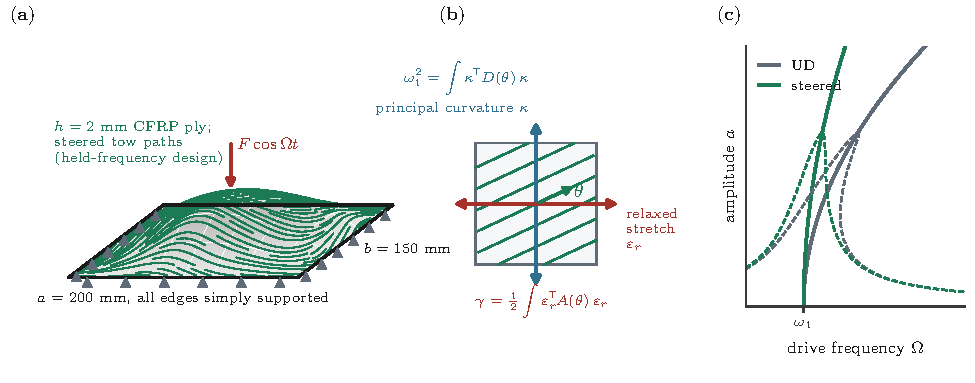
\includegraphics[width=\linewidth]{figs/fig_schematic.pdf}
\caption{The problem and the hypothesis. \textbf{(a)}~A simply supported
$200\times150\times2$\,mm CFRP plate, drawn deflected in its fundamental mode, with the tow
paths of the held-frequency steered design of Sec.~\ref{sec:levers} and the harmonic center
load. \textbf{(b)}~What one material point sees: the fiber direction $\theta$, the principal
curvature of the mode, which with the bending stiffness $\bm D(\theta)$ sets $\omega_1^2$, and
the principal relaxed stretch (drawn at the plate's typical $33^\circ$ conflict with the
curvature, Sec.~\ref{sec:mechanism}), which with the membrane stiffness $\bm A(\theta)$ sets
the hardening $\gamma$ (Sec.~\ref{sec:model}). \textbf{(c)}~The consequence, sketched: at the
same linear frequency $\omega_1$, a smaller hardening bends the backbone (solid) less, and the
forced response (dashed) of the unidirectional plate folds and jumps where the steered one
stays single-valued (Sec.~\ref{sec:jumpres}).}
\label{fig:schematic}
\end{figure}

\paragraph{Hypothesis.} (Fig.~\ref{fig:schematic}.) The linear frequency and the hardening
are integrals of the \emph{same} rotated stiffness tensor against two \emph{different}
strain fields of the fundamental mode. The frequency is set by the bending curvature,
$\omega_1^2=\int\bm\kappa^{\!\top}\bm D(\theta)\bm\kappa$. The hardening is set by the
membrane stretch the mode induces after the in-plane field has relaxed,
$\gamma=\tfrac12\int\bm\varepsilon_r^{\!\top}\bm A(\theta)\bm\varepsilon_r$
(Sec.~\ref{sec:model}). The two strain fields differ from point to point in magnitude
and in principal direction. We hypothesize that a spatially varying fiber angle can
therefore satisfy, \emph{pointwise}, a trade-off between the two energies that a uniform
angle can only satisfy \emph{on average}. Where stretching energy dominates, the fibers turn
across the principal stretch. Where bending energy dominates, they are set toward or away
from the principal curvature as the frequency constraint requires (away from it when the
frequency is held at the UD value, the lowest of all uniform layups). Stacking separates the
same two functionals in the classical way, through the thickness ($\bm D$ weights the outer
plies, $\bm A$ all plies equally \cite{tsai1968}); it is the competing freedom against which
the in-plane route is tested. Section~\ref{sec:theory} turns the hypothesis into precise
statements, which make five falsifiable predictions:
\begin{enumerate}[label=\textbf{P\arabic*},leftmargin=2.2em,itemsep=1pt]
\item An isotropic material offers no orientation lever at all
  (Corollary~\ref{cor:iso}).
\item For a single-ply beam, any uniform angle leaves the frequency-normalized hardening
  \emph{exactly} unchanged, so every gain must come from spatial variation. The
  optimal variation places compliant fibers where the mode does not bend: the inflection
  points (Proposition~\ref{prop:beam}).
\item On a plate, a steered field reaches combinations of linear frequency and hardening
  that no uniform layup reaches, whether a single angle or a stacking sequence.
\item The optimized orientation follows the local preferred directions of the two
  energies. A first-order pointwise design computed from the unidirectional mode alone
  already captures most of the gain (Proposition~\ref{prop:pointwise}).
\item The lever grows with the material anisotropy and with the conflict between the two
  strain fields, and is limited by the tow-curvature constraint relative to the length scale
  of those fields.
\end{enumerate}
\noindent A consequence follows if the predictions hold. The jump-free amplitude scales
as $J^{-1/2}$ (Proposition~\ref{prop:cusp}), so reducing the hardening at held frequency
widens the panel's hysteresis-free operating range by a predictable factor. That factor is a
property of the conservative backbone; the absolute thresholds also depend on damping and
forcing.

\subsection{Approach}
We test the predictions on a clamped laminated beam and on simply supported and clamped
laminated plates, all von K\'arm\'an. The backbone is computed by an SSM reduction verified
against analytic, harmonic-balance (EPMC) and finite-element references. For design we use
the SSM's hardening coefficient in a closed form that is exact for the in-plane relaxation
and evaluated on a \emph{mode-adaptive} fundamental, with an analytic adjoint. The plate
frequency is an equality constraint and the beam frequency a floor
($\omega_1\geq0.98\,\omega_{1,\UD}$). The tow-curvature limit is imposed pointwise. The
held-frequency plate design is then checked on refined bases, on an independent
finite-element model with the frequency re-matched, on the full multi-mode model (by its
SSM, by EPMC continuation and by time integration of up/down frequency sweeps), for other
supports, aspect ratios, damping laws and edge restraints, and under an as-built tow-defect
model.

\begin{center}
\fbox{\begin{minipage}{0.94\linewidth}\small
\textbf{What ``exact'' means in this paper.} Three levels are kept apart.
\emph{(i) Exact statements} are proved for the stated model class: the Fourier structure
(Proposition~\ref{prop:fourier}), isotropic annihilation (Corollary~\ref{cor:iso}), beam
invariance (Corollary~\ref{cor:beaminv}) and the UD floor among uniform laminates
(Corollary~\ref{cor:udfloor}). \emph{(ii) Exact within the discretized design model}: the
in-plane relaxation is exact for the adopted von K\'arm\'an kinematics and in-plane basis
(Proposition~\ref{prop:relaxed}), and the frequency equality holds to $10^{-10}$ on the design
basis. \emph{(iii) Approximate across models}: on finer bases and an independent finite-element
model, the steered frequency differs from the UD value by up to $\nHeldTol\%$. We therefore also
report the hardening ratio with the frequency re-matched in each of those models
(Sec.~\ref{sec:confirm}). The cubic backbone itself is a small-amplitude approximation, valid
over the amplitude range verified against full-order EPMC (Appendix~\ref{app:calib}).
\end{minipage}}
\end{center}

\paragraph{Organization.} Section~\ref{sec:model} states the model, the reduction and the
backbone and jump quantities. Section~\ref{sec:theory} develops the mechanism and its
predictions. Section~\ref{sec:design} poses the design problem and derives its
sensitivities. Section~\ref{sec:results} tests P1--P5, the robustness of the result and the
consequence for the forced response. Section~\ref{sec:discussion} states what the results do
and do not establish. The appendices give the SSM recursion, the SSM--condensation
equivalence, the finite-element validation, calibration against prior work, and a
verification and reproducibility map.
